\documentclass{beamer}
\usetheme{Warsaw}
\usepackage{tikz}

\usebackgroundtemplate{%
	\tikz\node[opacity=0.2] {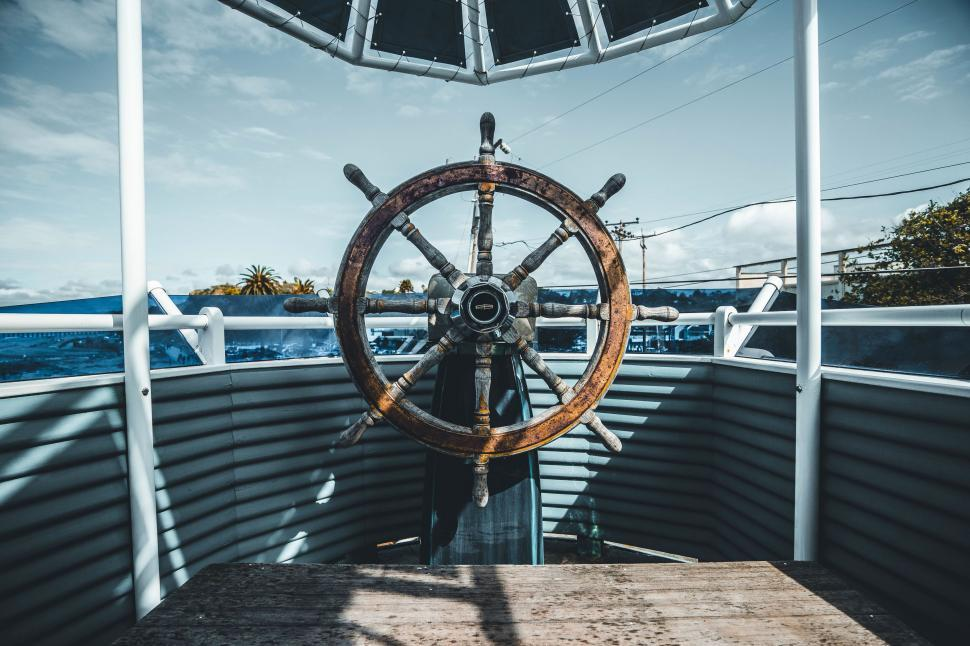
\includegraphics[height=\paperheight]{ship_helm.jpg}};}
\title{Beginning Kubernetes}
\author{Jacob W. Archambault}
\institute{SAIC}
\AtBeginSubsection[]
{
	\begin{frame}<beamer>{Outline}
		\tableofcontents[currentsection, currentsubsection]
	\end{frame}
}

\begin{document}
	\begin{frame}[plain]
		\titlepage
	\end{frame}
	\begin{frame}{Outline}
		\tableofcontents[pausesections]
		% You might wish to add the option [pausesections]
	\end{frame}
	\section{What Kubernetes is}
	\begin{frame}{What Kubernetes is}
		\begin{itemize}
			\item An \href{https://github.com/kubernetes/kubernetes}{open source} system for automating deployment, scaling, and management of containerized applications.
			\pause
			\item An open source system for managing containerized applications across multiple hosts.
			\pause
			\item An open-source container orchestration platform.
		\end{itemize}
	\end{frame}
	\subsection{Containers 101}
	\begin{frame}{Container images}
		\begin{itemize}
			\item created from a Containerfile (usually)
			\pause
			\item can also be created from a running image via \texttt{docker commit}
		\end{itemize}
	\end{frame}
	\begin{frame}{Containers 101}
		\begin{itemize}
			\item an isolated runnable instance of an image 
			\pause 
			\item achieves isolation via Linux \textit{namespaces}
			\pause
			\item limits resource usage (e.g. CPU usage) via Linux \textit{cgroups}
		\end{itemize}
	\end{frame}
	\begin{frame}{How containers differ from VMs}
		\begin{itemize}
			\item more lightweight and portable than AMI images
			\pause
			\item requires a machine to run on, called \textit{nodes} in K8s
		\end{itemize}
	\end{frame}
	\subsection{Container orchestration}
	\begin{frame}{What is orchestration}
		\begin{itemize}
			\item Orchestration - managing the scaling and deployment of multiple containers across potentially many nodes
		\end{itemize}
	\end{frame}
	
	\section{Why use Kubernetes}
	\begin{frame}{Why use Kubernetes}
		Yes
	\end{frame}
	\section{Where to use Kubernetes}
	\begin{frame}{Where to use Kubernetes: Cloud providers}
		\begin{itemize}
			\item Google Cloud - Google Kubernetes Engine (GKE)
			\pause
			\item Azure - Azure Kubernetes Service (AKS)
			\pause
			\item AWS Elastic Kubernetes Service (EKS)
		\end{itemize}
	\end{frame}
	\begin{frame}{Where to use Kubernetes: Local environment}
		\begin{itemize}
			\item Docker Desktop
			\pause
			\item \texttt{podman kube}
			\pause
			\item minikube
		\end{itemize}
	\end{frame}
	\section{When not to use Kubernetes}
	\begin{frame}
		\begin{itemize}
			\item static websites (S3 with CloudFront/load balancing)
			\item single container applications (Azure App Service, Elastic Beanstalk)
		\end{itemize}
		
	\end{frame}
	\section{When to use Kubernetes}
	\begin{frame}{When to use Kubernetes}
		\begin{itemize}
			\item Multi-cloud environments to avoid vendor lock-in
			\pause
			\item Applications involving dozens or hundreds of interdependent services
			\pause
			\item Integrating non-cloud-specific services via Helm
		\end{itemize}
	\end{frame}
	\section{Kubernetes components}
	\subsection{Kubernetes components: compute}
	\begin{frame}{Kubernetes components: Pods}
		\begin{itemize}
			\item one or more containers with shared resources and networking			
		\end{itemize}
	\end{frame}
	\begin{frame}{Kubernetes components: ReplicaSets}
		\begin{itemize}
			\item A specified number of a set of pods			
		\end{itemize}
	\end{frame}
	\begin{frame}{Kubernetes components: Deployments}
		\begin{itemize}
			\item A deployment manages a ReplicaSet, ensuring that the desired number of pods is maintained and that pods are healthy
		\end{itemize}
	\end{frame}
	\subsection{Kubernetes components: storage}
	\begin{frame}{Volumes and Volume claims}
		\begin{itemize}
			\item A PersistentVolume is an actual data storage entities created and used by deployments
			\pause
			\item PersistentVolumeClaim is a request for storage by a user
		\end{itemize}
	\end{frame}
	\subsection{Other Kubernetes component types}
	\begin{frame}
		\begin{itemize}
			\item Configuration: ConfigMaps and Secrets
			\pause
			\item Finite tasks: Jobs and CronJobs
		\end{itemize}
	\end{frame}
	\section{Conclusion}
	\begin{frame}[plain]
		\titlepage
	\end{frame}
\end{document}
